\documentclass{article}

% Language setting
\usepackage[english]{babel}

% Set page size and margins
% Replace `letterpaper' with `a4paper' for UK/EU standard size
\usepackage[letterpaper,top=2cm,bottom=2cm,left=3cm,right=3cm,marginparwidth=1.75cm]{geometry}

% Useful packages
\usepackage{amsmath}
% --- Code listings ---
\usepackage{listings}
\usepackage{xcolor}
\definecolor{codegreen}{rgb}{0,0.6,0}
\definecolor{codegray}{rgb}{0.5,0.5,0.5}
\definecolor{codepurple}{rgb}{0.58,0,0.82}
\definecolor{backcolour}{rgb}{0.95,0.95,0.92}

\lstdefinestyle{mystyle}{
    backgroundcolor=\color{backcolour},   
    commentstyle=\color{codegreen},
    keywordstyle=\color{magenta},
    numberstyle=\tiny\color{codegray},
    stringstyle=\color{codepurple},
    basicstyle=\ttfamily\footnotesize,
    breakatwhitespace=false,         
    breaklines=true,                 
    captionpos=b,                    
    keepspaces=true,                 
    numbers=left,                    
    numbersep=5pt,                  
    showspaces=false,                
    showstringspaces=false,
    showtabs=false,                  
    tabsize=2
}

\lstset{style=mystyle}
% --- End Code Listings
\usepackage{graphicx}
\usepackage{float}
% \usepackage{caption}
% \usepackage{subcaption}
\usepackage[colorlinks=true, allcolors=blue]{hyperref}
\graphicspath{{./figures/}}

\title{ECE 637 - Lab 1}
\author{Colin Braun}

\begin{document}
\maketitle

\section{Power Spectral Density of an Image}
\subsection{The gray scale image img04g.tif}
\begin{figure}[H]
    \centering
    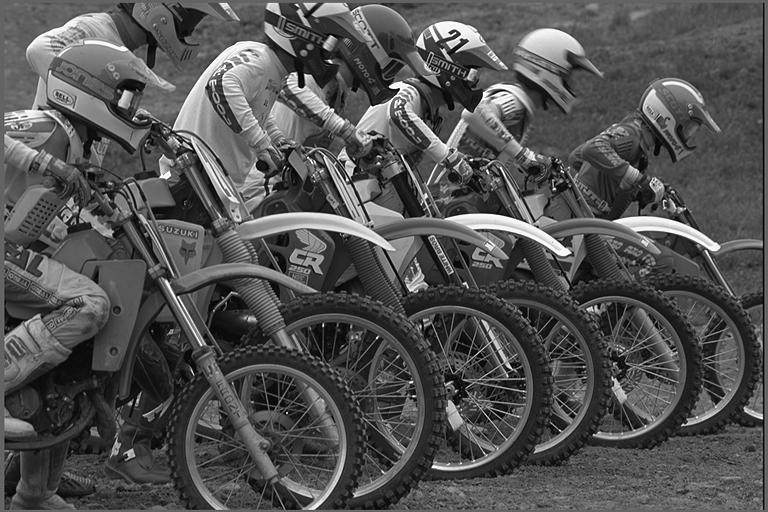
\includegraphics[width=1\textwidth]{../images/img04g.png}
    \begin{center}
    \end{center}
\end{figure}
\subsection{The power spectral density plots for block sizes of 64 × 64, 128 × 128, and 256 × 256}
\begin{figure}[H]
    \centering
    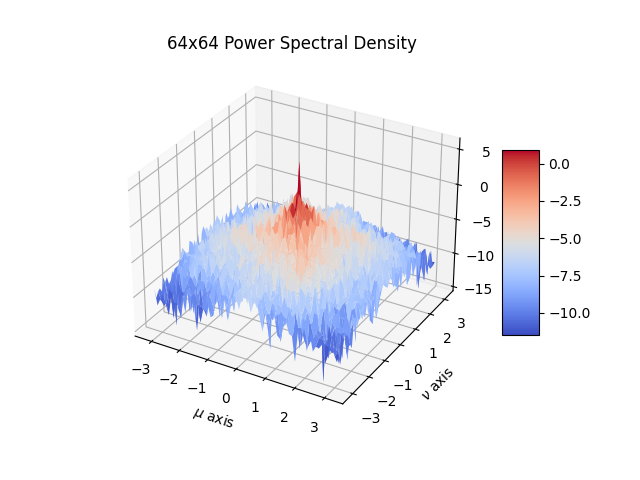
\includegraphics[width=0.75\textwidth]{../images/log-pwr-spec-density-64x64.png}
    \begin{center}
    \end{center}
\end{figure}
\begin{figure}[H]
    \centering
    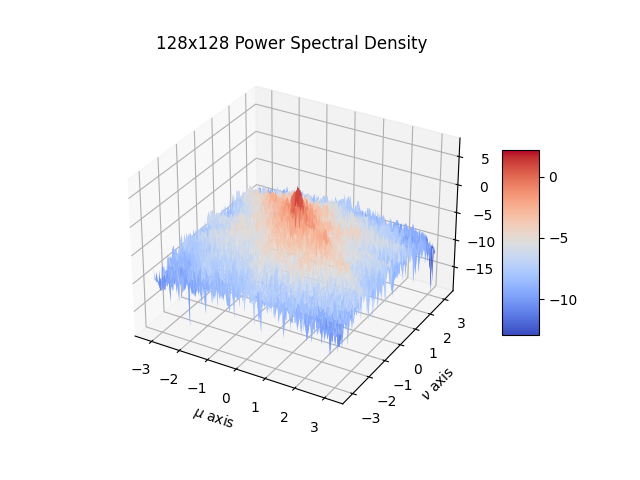
\includegraphics[width=0.75\textwidth]{../images/log-pwr-spec-density-128x128.png}
    \begin{center}
    \end{center}
\end{figure}
\begin{figure}[H]
    \centering
    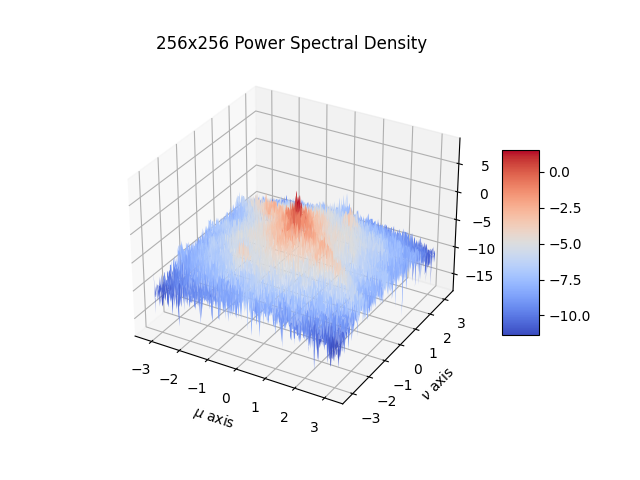
\includegraphics[width=0.75\textwidth]{../images/log-pwr-spec-density-256x256.png}
    \begin{center}
    \end{center}
\end{figure}
\subsection{The improved power spectral density estimate.}
\begin{figure}[H]
    \centering
    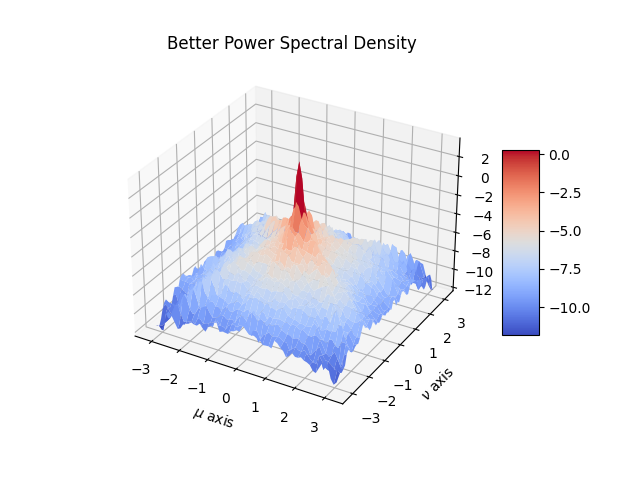
\includegraphics[width=0.75\textwidth]{../images/log-pwr-spec-density-better.png}
    \begin{center}
    \end{center}
\end{figure}
\subsection{Code for BetterSpecAnal(x) function}
\lstinputlisting[language=Python, firstline=13, lastline=39]{../SpecAnal.py}



\section{Power Spectral Density of a 2-D AR Process}
\subsection{The image 255 * (x + 0.5)}
\begin{figure}[H]
    \centering
    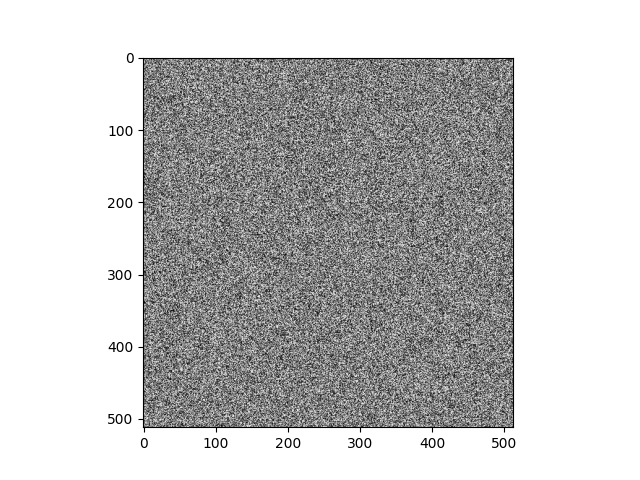
\includegraphics[width=0.75\textwidth]{../images/np-rand-uniform.png}
    \begin{center}
    \end{center}
\end{figure}
\subsection{The image y + 127}
\begin{figure}[H]
    \centering
    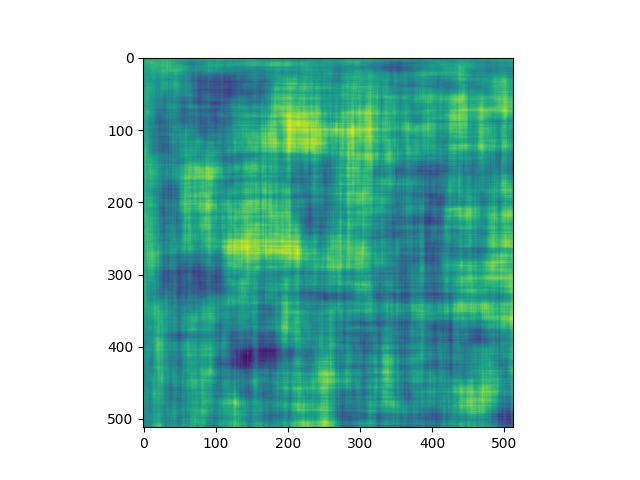
\includegraphics[width=0.75\textwidth]{../images/image-p-127.png}
    \begin{center}
    \end{center}
\end{figure}
\subsection{A mesh plot of the function log $S_y(e^{j\mu}, e^{j\nu})$}
\begin{figure}[H]
    \centering
    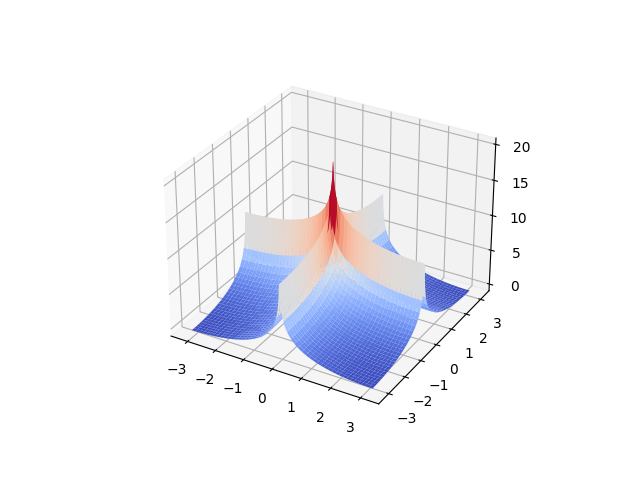
\includegraphics[width=0.75\textwidth]{../images/y-log-pwr-spec-density-theoretical.png}
    \begin{center}
    \end{center}
\end{figure}
\subsection{A mesh plot of the log of the estimated power spectral density of y using BetterSpecAnal(y)}
\begin{figure}[H]
    \centering
    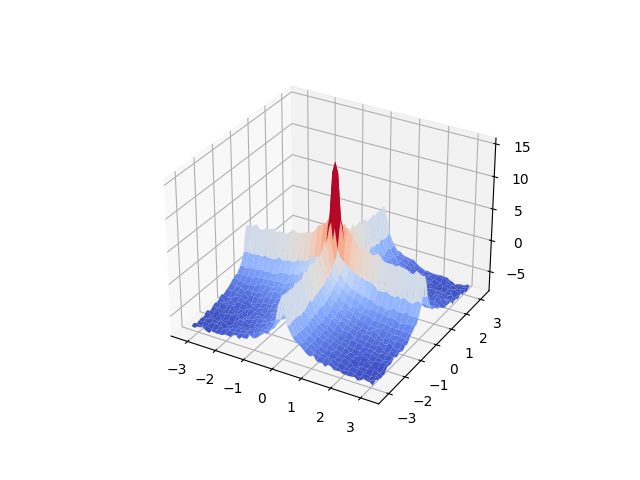
\includegraphics[width=0.75\textwidth]{../images/y-log-pwr-spec-density-better.png}
    \begin{center}
    \end{center}
\end{figure}

\end{document}
